% !TeX root = ../note.tex
\section{Тестирование}\label{sec:testing}

Для тестирования работы сервисов будут использоваться два типа тестов: интеграционные и юнит-тесты. Критически важно покрыть тестами механизм матчинга ордеров биржи, так как от этого зависит правильный обмен средств между клиентами, и в случае ошибки организации-владельцу биржи придётся возмещать убытки клиентов из собственных средств.

\subsection{Юнит-тестирование}

Это процесс, позволяющий проверить на корректность отдельные модули исходного кода программы, наборы из одного или более программных модулей вместе с соответствующими управляющими данными, процедурами использования и обработки.

Идея состоит в том, чтобы писать тесты для каждой нетривиальной функции или метода. Это позволяет достаточно быстро проверить, не привело ли очередное изменение кода к регрессии, то есть к появлению ошибок в уже протестированных местах программы, а также облегчает обнаружение и устранение таких ошибок.

Тесты в матчинг сервисе можно разделить на два больших блока: тесты на парный матчинг и тесты на матчинг нескольких ордеров.

Тесты на парный матчинг проверяют корректность матчинга двух ордеров для каждой возможной совокупности параметров ордеров: цены, объёма и времени появления одного ордера с ценой, объёмом и временем появления  другого ордера.

Возможные совокупности параметров:
\begin{enumerate}
    \item Первым создан ордер на покупку: цена — выше, объём — выше.
    \item Первым создан ордер на покупку: цена — выше, объём — ниже.
    \item Первым создан ордер на покупку: цена — выше, объём — равный.
    \item Первым создан ордер на покупку: цена — ниже, объём — выше.
    \item Первым создан ордер на покупку: цена — ниже, объём — ниже.
    \item Первым создан ордер на покупку: цена — ниже, объём — равный.
    \item Первым создан ордер на покупку: цена — равная, объём — выше.
    \item Первым создан ордер на покупку: цена — равная, объём — ниже.
    \item Первым создан ордер на покупку: цена — равная, объём — равный.
    \item Первым создан ордер на продажу: цена — выше, объём — выше.
    \item Первым создан ордер на продажу: цена — выше, объём — ниже.
    \item Первым создан ордер на продажу: цена — выше, объём — равный.
    \item Первым создан ордер на продажу: цена — ниже, объём — выше.
    \item Первым создан ордер на продажу: цена — ниже, объём — ниже.
    \item Первым создан ордер на продажу: цена — ниже, объём — равный.
    \item Первым создан ордер на продажу: цена — равная, объём — выше.
    \item Первым создан ордер на продажу: цена — равная, объём — ниже.
    \item Первым создан ордер на продажу: цена — равная, объём — равный.
\end{enumerate}

Для каждого случая подбирается подбираются параметры и рассчитывается результат матчинга. Параметры подбираются с учётом крайних значений, чтобы тесты одновременно проверяли работоспособность матчинга на неудобных значениях. Так как все тесты этой категории проходят по одному сценарию, был написан общий шаблон для всех. Пример теста приведён на рисунке~\ref{fig:unit_test}.

\begin{figure}[ht]
    \centering
    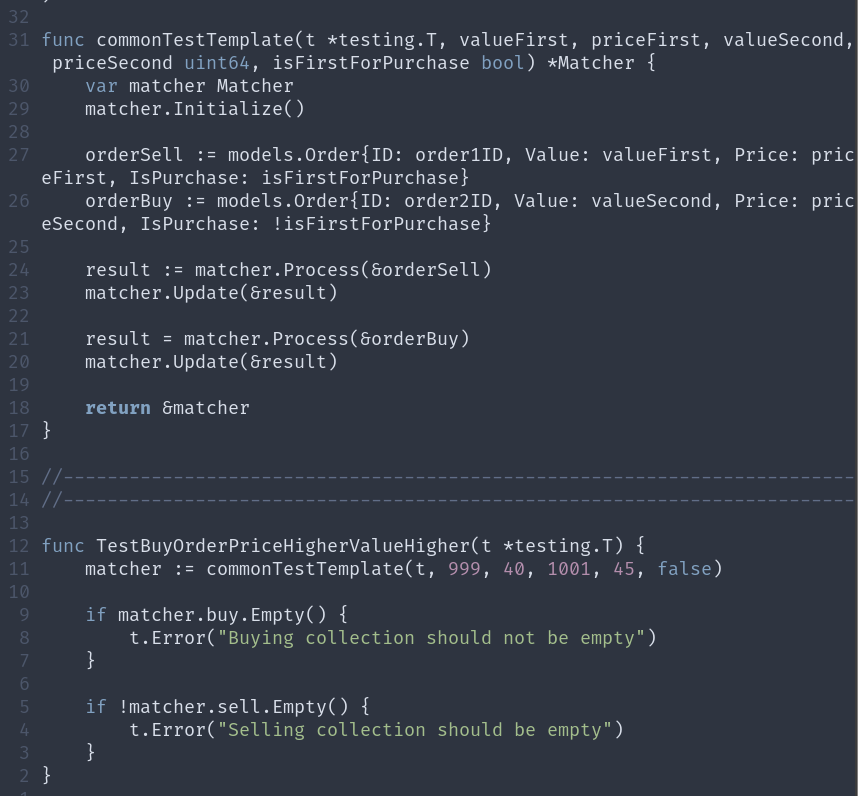
\includegraphics[width=\textwidth]{tests1}
    \caption{Юнит-тест для матчинга}\label{fig:unit_test}
\end{figure}

Данный тест проверяет первый случай из списка выше, когда первым создан ордер на покупку, с более высокой ценой, и большим объёмом. В результате теста ордеры должны закрыть друг друга. Проверяется это через количество открытых ордеров в коллекциях ордеров на продажу или покупку. Если после очередного изменения кода что-то сломается и коллекция ордеров на продажу не очистится или наоборот, коллекция ордеров на покупку станет пустой, то будут выброшены соответствующие ошибки.

Тесты на матчинг нескольких ордеров сложнее в написании так как у них различаются сценарии исполнения. Пример теста приведён на рисунке~\ref{fig:unit_test2}

\begin{figure}[ht]
    \centering
    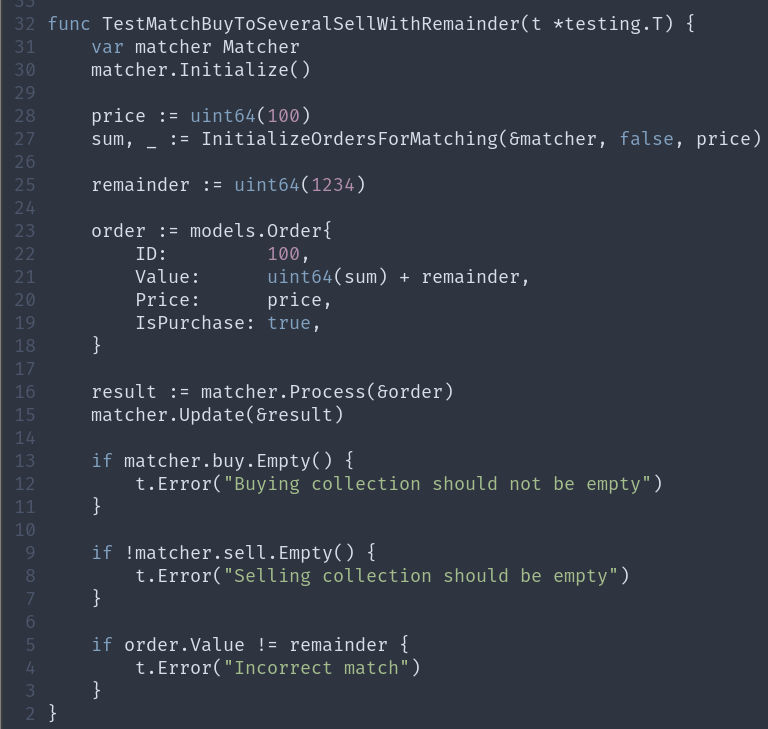
\includegraphics[width=\textwidth]{tests2}
    \caption{Юнит-тест нескольких ордеров для матчинга}\label{fig:unit_test2}
\end{figure}

Данный тест проверяет матчинг одного большого ордера на покупку с несколькими маленькими ордерами на продажу при условии, что общая сумма, выставленная на продажу в соответствующих ордерах меньше, чем сумма, которую хочет купить ордер на покупку. То есть подразумевается наличие некоторого остатка на ордере, значит ордер не должен закрыться после матчинга со всеми остальными ордерами. Кроме самого наличия незакрытого ордера, проверяется также сумма остатка этого ордера.
На рисунке~\ref{fig:testsresult} представлен результат запуска всех юнит-тестов:

\begin{figure}[ht]
    \centering
    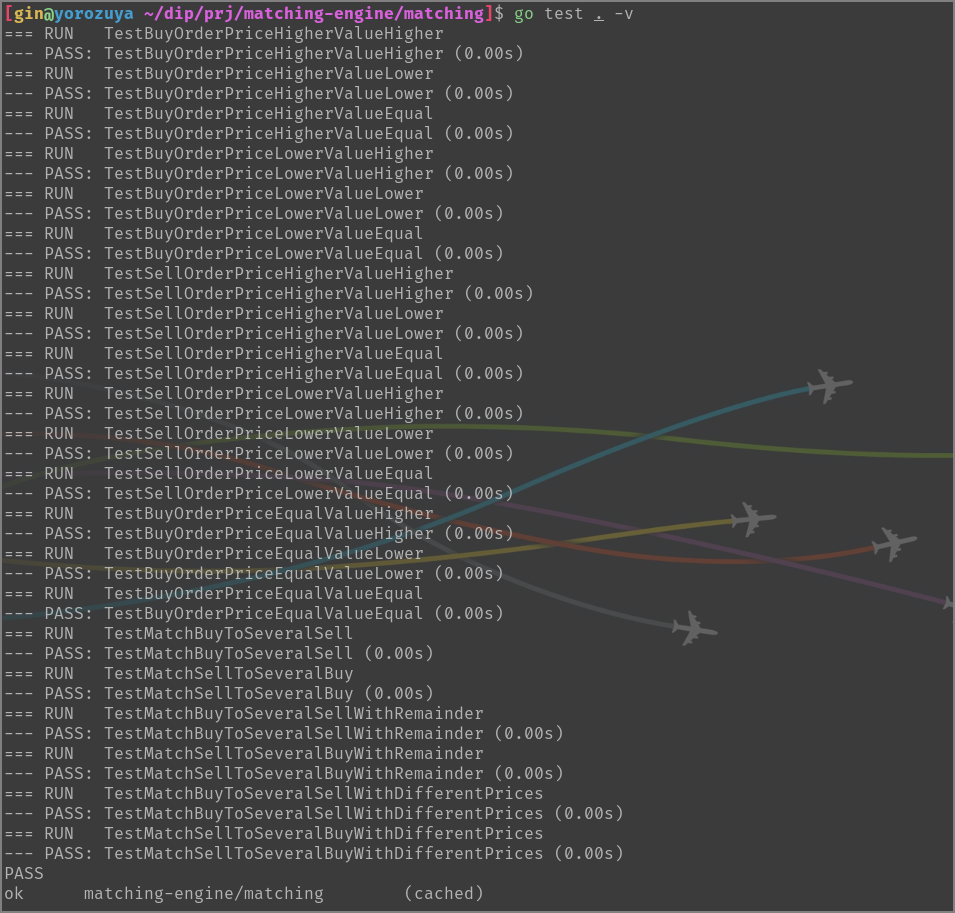
\includegraphics[width=\textwidth]{testsresult}
    \caption{Результаты юнит-тестирования}\label{fig:testsresult}
\end{figure}

Исходя из полученного успешного результата тестирования можно сделать вывод, что механизм матчинга на момент запуска тестов находится в рабочем состоянии.

\subsection{Интеграционное тестирование}

Также было проведено интеграционное тестирование проекта. Для этих целей был написан модуль тестирования, включающий в себя обёртки над клиентами для баз данных, событий и очереди сообщений. Модуль работает в два потока. Один из потоков является управляющим, считает количество пройденных успешно тестов и показывает ошибки непройденных тестов. Второй поток постоянно перезапускается с новым тестом и выбрасывает ошибку, если тест провалится. Второй поток для теста необходим, так как ошибку вида \lstinline[language=Golang]{panic()} в Golang отловить нельзя, но можно обработать и передать результат в другой поток.

На листинге~\ref{list:itester} приведен код главного модуля тестирования.

\lstinputlisting[caption=Структура модуля тестирования,language=Golang,label={list:itester}]{appendix/itester.go}

Модуль тестирования состоит из:
\begin{itemize}
    \item Обёртки над клиентами MongoDB, Clickhouse, Redis и RabbitMQ;
    \item Регулярное выражение для запуска тех тестов, которые подходят под шаблон в выражении;
    \item Поля для хранения названия и функции для текущего исполняемого теста;
    \item Флаги для пометки теста завершённым и провалившимся.
\end{itemize}

Все тесты выполняются поочерёдно. При наличии провалившегося теста будет выведена ошибка, и тесты продолжат выполняться. Алгоритм выполнения тестов в модуле:

\begin{enumerate}
    \item Считывание названий тестов и функций самих тестов;
    \item Подключение модуля ко всем внешним сервисам, необходимым для работы сервиса;
    \item Запуск цикла тестирования;
    \item Проверка названия теста по шаблону из модуля. Если название подходит, то запускается сам тест;
    \item Очистка данных в сервисах, в том случае, когда идёт запуск не первого теста;
    \item Запуск матчинг-сервиса;
    \item Запуск теста и ожидание результатов выполнения;
    \item После завершения всех тестов закрывается подключение ко всем сервисам.
\end{enumerate}

Пример интеграционного теста приведён в приложении~А. В тесте имитируется матчинг нескольких ордеров на покупку и одного ордера на продажи, когда суммарные средства ордеров на покупку равны средствам ордера на продажу. В тесте создаются ордера, которые посылаются в канал RabbitMQ, затем проверяются события из Redis о матчинге, а также записи в MongoDB и Clickhouse и новых ордерах и сделках.

Результат интеграционного тестирования с названиями пройденных тестов, представлены ни рисунке~\ref{fig:itestlog}

\begin{figure}[ht]
    \centering
    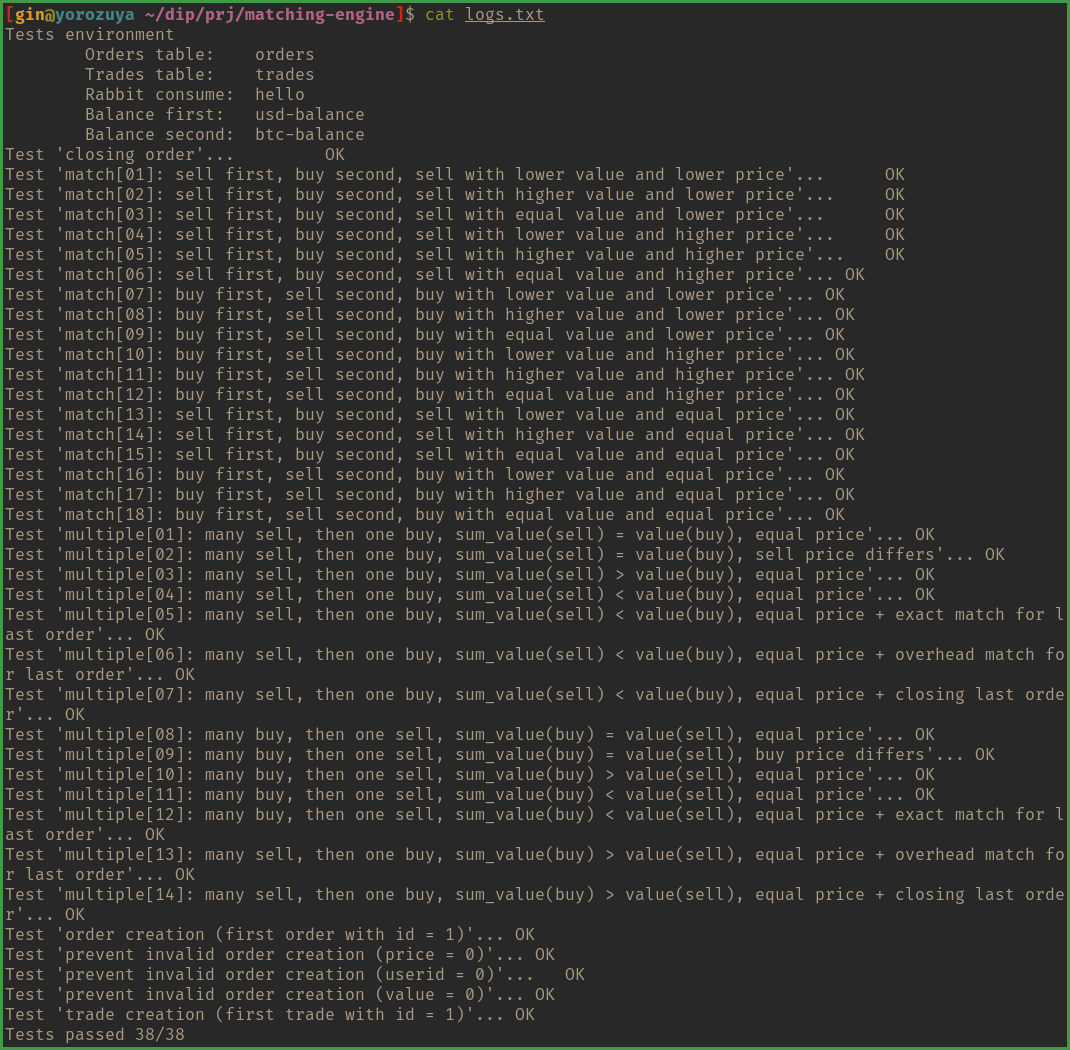
\includegraphics[width=\textwidth]{itestlog}
    \caption{Результаты интеграционного тестирования}\label{fig:itestlog}
\end{figure}

По результатам проведённого интеграционного и юнит-тестирования можно сказать, что программный продукт написан достаточно качественно и проведённое тестирование сделано довольно обширно. В будущем возможно написание дополнительных тестов при расширении функционала сервиса, а также дополнительное тестирование сервиса авторизации.
